%#####################################################################################################################
% Datei	: MSec.tex
% Autor	: Byron Worms
%#####################################################################################################################
% Dokumenteinstellungen
\documentclass[conference]{acmsiggraph}

% Umlaute etc..
\usepackage[latin1]{inputenc}						
\usepackage[T1]{fontenc}

% Bibliothek f�r das Quellenverzeichnisse
\let\bibhang\relax
\usepackage[style=alphabetic,backend=biber,sorting=none]{biblatex}
\addbibresource{Literaturverzeichnis.bib}
\renewcommand{\bibfont}{\small}

% Bilder unterst�tzen
\usepackage[]{graphicx}

% PDF Inkludierung unterst�tzen
\usepackage{pdfpages}

% Farben unterst�tzen
\usepackage{xcolor}
\usepackage{color}
\usepackage{colortbl}

% Verweise auf Title
\usepackage{titleref}

% Sprachunterst�tzung (Letzte Sprache wird als Richtlinie genutzt!)
\usepackage[english,ngerman]{babel}
\usepackage{csquotes}

% Symbolunterst�tzung wie €
\usepackage{textcomp}

% Anhang unterst�tzen
\usepackage[titletoc]{appendix}

% Erweiterte Fu�noten unterst�tzen
\usepackage[hang]{footmisc}
\setlength{\footnotemargin}{1em}

% Unterst�tzung mehrzeiliger Kommentare
\usepackage{comment}

% Erweiterte Tabellen unterst�tzen
\usepackage{booktabs}
\usepackage{tabularx}
\usepackage{tabulary}
\usepackage{longtable,tabu}
\usepackage{array}

% Mathematische Operationen in {} Ausdr�cken erlauben (z.B. {\linewidth-4cm})
\usepackage{calc}

% "float" Positionierung unterst�tzen
\usepackage{scrhack}
\usepackage{float}

% Erweiterte Aufz�hlungen unterst�tzen
\usepackage{enumitem}

% Erweiterte Tabellenlinien unterst�tzen
\usepackage{hhline,float}

% Rotationen unterst�tzen
\usepackage{rotating}

% Erweiterte Symbole unterst�tzen
\usepackage{bbding} 
\usepackage{dingbat}
\usepackage{wasysym}
\usepackage{amssymb}

% Begrenzungsrahmen anzeigen lassen
%\usepackage{showframe}

% Tabellen werden nicht von Latex neupositioniert
\restylefloat{table}

% Bilder werden nicht von Latex neupositioniert
\restylefloat{figure}

% PDF Version 1.6 erzwingen
\pdfminorversion=6

% Kompression setzen (hyperref setzt das Level auf 9!)
\pdfcompresslevel=9

% Verschiebungen und Formattierungen des Modus "twoside" aufheben
\raggedbottom

% Diverse Hilfsfunktionen
\newcommand{\boldT}{\normalfont \bfseries}
\newcommand{\boldtext}[1]{{\normalfont \bfseries {#1}}}

% Eigene Definition von "\toprule" und "\bottomrule".
% Verhindert den Abstand zwischen den beiden Linien und den Vertikalen
\newcommand{\mytoprule}{\specialrule{1.25pt}{0em}{0em}}
\newcommand{\mybottomrule}{\specialrule{1.25pt}{0em}{0em}}
\newcommand{\mytoprulehalf}{\specialrule{0.75pt}{0em}{0em}}
\newcommand{\mybottomrulehalf}{\specialrule{0.75pt}{0em}{0em}}

% Eigene Definition f�r das Einbinden von Grafiken (erzeugt automatisch einen Rahmen um die Grafik)
% Bsp: \framepicture[width=0.5\textwidth, page=1]{...}
\newcommand{\framepicture}[2][\empty]{\fbox{\includegraphics[#1]{#2}}}

% Definierte Farben
\definecolor{mygreen}{rgb}{0.7,0.9,0.11}
\definecolor{myorange}{rgb}{1.0,0.49,0.15}

% Titel und Autoren festlegen
\title{SS15 Topic 05: Perceptual Hashing of Images}
\author{
	Byron Worms\\
	Multimedia and Security\\
	Fakult�t f�r Informatik\\
	byron.worms@st.ovgu.de
	}
\pdfauthor{Byron Worms}

% Schlagw�rter festlegen
\keywords{multimedia, security, hashing, perceptual, images, hash, robust hash, fingerprint}

%---------------------------------------------------------------------------------------------------------------------
% Einstiegspunkt
%---------------------------------------------------------------------------------------------------------------------
\begin{document}
	\maketitle						% Title generieren
	%#####################################################################################################################
% Datei	: Abstract.tex
% Autor	: Byron Worms
%#####################################################################################################################
\section*{Kurzfassung}
Das vorliegende technische Paper untersucht einen alternativen Ansatz der Authentifizierungs-- und Integrit�tspr�fung
von unterschiedlichen Bildmaterial mittels \textit{Perceptual Hashing} unter der Verwendung vor vier verschiedenen
Algorithmen.
\\
F�r die eingehende Analyse des Ansatzes wird ein gro�es Spektrum an variierenden Testdaten definiert und in Bezug
auf die Algorithmen hin diskutiert. Mit Hilfe der divergierenden Experimente soll eine m�gliche Korrelation zwischen
den resultierenden Erkennungs-- sowie Fehlerraten der einzelnen Verfahren und dem differenzierenden Bildmaterial analysiert
werden.
\\
Ein weiterer Untersuchungspunkt der Arbeit beschreibt die potentielle Effizienzsteigerung bei der Verwendung von
Algorithmen aus dem Bereich \textit{Perceptual Hashing} gegen�ber nativen Vergleichsans�tzen.
			% Abstrakt einbinden	
	\keywordlist					% Keywords ausgeben
	\copyrightspace					% Copyright-Sektion generieren
	%................................................................
	% Ab hier den eigentlichen Inhalt einf�gen
	%#####################################################################################################################
% Datei	: Introduction.tex
% Autor	: Byron Worms
%#####################################################################################################################
%---------------------------------------------------------------------------------------------------------------------
% Motivation
%---------------------------------------------------------------------------------------------------------------------
\section{Motivation}
\label{sec:motivation}
ToDo

%---------------------------------------------------------------------------------------------------------------------
% Description of the used approach
%---------------------------------------------------------------------------------------------------------------------
\section{Perceptual Hashing of Images}
ToDo
		% Einleitung einbinden
	%#####################################################################################################################
% Datei	: TaskDescription.tex
% Autor	: Byron Worms
%#####################################################################################################################
%---------------------------------------------------------------------------------------------------------------------
% Problem description and investigation tasks
%---------------------------------------------------------------------------------------------------------------------
\section{Problembeschreibung}
\label{sec:tasks}
ToDo
	% Aufgabenstellung einbinden
	%#####################################################################################################################
% Datei	: Solution.tex
% Autor	: Byron Worms
%#####################################################################################################################
%---------------------------------------------------------------------------------------------------------------------
% Solution approach
%---------------------------------------------------------------------------------------------------------------------
\section{L�sungsansatz}
\label{sec:solution}
F�r das Verst�ndnis grundlegender Funktionsweisen der verschiedenen Algorithmen und der Auswahl des
variierenden Bildmaterials, ist ein Basiswissen �ber den allgemeinen Aufbau von Bildern und deren digitale Repr�sentation 
erforderlich.
\\
In Abh�ngigkeit des gew�hlten Farbmodells werden Bilder oftmals durch eine Koeffizientenmatrix von Helligkeitswerten
beschrieben. Im Beispiel des RGB--Farbmodells ist die finale Pixelfarbe durch drei unterschiedliche Koeffizienten der
einzelnen Farbkan�le (rot, gr�n und blau) definiert, wohingegen ein Graustufenbild nur einen Farbkanal besitzt.
\\
Die Konkretisierung einer gegebenen Matrix aus Koeffizienten erzeugt dabei ein digitales Bild und/oder Muster, 
das strukturell in sowohl hochfrequente als auch in niederfrequente Bereiche unterteilt ist. Gleichm��ige Unterschiede innerhalb
der Bildstruktur werden durch die niederfrequenten Anteile abgebildet, wohingegen hochfrequente Bestandteile mit ungleichm��igen
und pl�tzlichen strukturellen �nderungen zum Detail des Gesamtbilds beitragen.

\subsection{Testdaten}
\label{sec:solution_testdata}
Das verwendete Bildmaterial ist in die drei unten aufgef�hrten Kategorien eingeteilt. Die Unterteilung des Gesamtdatensatzes
dient einer Komplexit�t abh�ngigen, verbesserten Erkenntnisgewinnung der jeweiligen Arbeitsweisen der verschiedenen eingesetzten
Algorithmen. Somit soll ein Zusammenspiel zwischen den Fehlerkennungen der Algorithmen und dem strukturellen Aufbau der
Bilder leichter detektiert werden.

\boldtext{Einfache Farben}\\
Diese Kategorie beinhaltet neun verschiedenfarbige Bilder mit den in der Tabelle~\ref{tab:solution_simplecolors_specs} stehenden
Spezifikationen. Der Farbbereich deckt dabei sowohl helle als auch dunkle Farben ab.
\begin{table}[H]
	\begin{center}
		\begin{tabular}{|l|c|}
			\mytoprule
			\centering\bfseries Eigenschaft & Wert(e)
			\\
			\hline
			\hline
			%---------------------------------------------------------------------------------------------------------------------	
			\textit{Kodierung} & JPEG, 100\% Qualit�t
			\\
			\hline
			%---------------------------------------------------------------------------------------------------------------------	
			\textit{Aufl�sung} & 600x600px
			\\																				
			%---------------------------------------------------------------------------------------------------------------------
			\mybottomrule			
		\end{tabular}
		\caption{Spezifikationen \textit{Einfache Farben} (Eigene Darstellung)}
		\label{tab:solution_simplecolors_specs}
	\end{center}
\end{table}

\boldtext{Elementare Formen}\\
Die Kategorie ist in drei unterschiedliche Gruppen mit je 54 Bildern eingeteilt, wobei die Bildmotive abh�ngig von der
Gruppierung variieren. Die nachfolgenden Abbildung~\ref{fig:solution_brushes} schafft einen �berblick �ber die verwendeten Muster
in den jeweiligen Gruppen. Die Farben der elementaren Formen sind dabei identisch zu den Farbwerten aus der Kategorie
\textit{Einfache Farben}.
\begin{figure}[H]
	\centering
	\framepicture[width=0.96\linewidth]{Pictures/simple_brushes.png}
	\caption{Gruppierung der elementaren Formen (Eigene Darstellung)}
	\label{fig:solution_brushes}
\end{figure}
\noindent
Die drei Gruppen umfassen neben den Originalbildern ebenfalls durch Filter ver�ndertes Bildmaterial. Folgende
�nderungen sind auf die originalen Bilder angewendet worden: \textit{Skalierungs�nderungen, Rotationen, Gammaanpassungen und Rauschen}.
Die Bildspezifikationen sind identisch zu denen aus der Kategorie \textit{Einfache Farben}. Die genaue Parametrisierung der Filter
ist dabei dem Anhang~\ref{sec:appendix_b} (\textit{Dokumentation der verwendeten Daten}) zu entnehmen.

\boldtext{Komplexe Bilder}\\
Die komplexen Bilder sind �hnlich zu der Kategorie \textit{Elementare Formen}. Diese beinhaltet jedoch nur eine Gruppe mit 21 verschieden
�hnlichen sowie nicht �hnlichen Fotos, welche die in Tabelle~\ref{tab:solution_images_specs} stehenden Spezifikationen aufweisen:
\begin{table}[H]
	\begin{center}
		\begin{tabular}{|l|c|}
			\mytoprule
			\centering\bfseries Eigenschaft & Wert(e)
			\\
			\hline
			\hline
			%---------------------------------------------------------------------------------------------------------------------	
			\textit{Kodierung} & JPEG, 100\% Qualit�t
			\\
			\hline
			%---------------------------------------------------------------------------------------------------------------------	
			\textit{Aufl�sung} & 1024x768px
			\\																				
			%---------------------------------------------------------------------------------------------------------------------
			\mybottomrule			
		\end{tabular}
		\caption{Spezifikationen \textit{Komplexe Bilder} (Eigene Darstellung)}
		\label{tab:solution_images_specs}
	\end{center}
\end{table}
Die �nderungen mittels Filter entsprechen den Anpassungen aus der Kategorie \textit{Elementare Formen}.

\subsection{Algorithmen}
\label{sec:solution_algorithms}
Alle vier in der \textit{Problemstellung} erw�hnten Algorithmen arbeiten f�r die Berechnung eines robusten Hashes auf dem
strukturellen Inhalt des Bildmaterials. Die verschiedenen Vorgehensweisen bei der Extraktion der erforderlichen Merkmale sowie
der anschlie�ende Vergleich der errechneten Hashwerte kann mit der nachfolgenden Tabelle~\ref{tab:solution_algorithms}
zusammengefasst werden:
\begin{table}[H]
	\begin{center}
		\begin{tabular}{|l|c|c|}
			\mytoprule
			\centering\bfseries Algorithmus & \bfseries Hashl�nge & \bfseries Vergleichsverfahren
			\\
			\hline
			\hline
			%---------------------------------------------------------------------------------------------------------------------	
			DCT & 64 Bit & Hamming Distanz
			\\
			\hline
			%---------------------------------------------------------------------------------------------------------------------	
			RADISH & 320 Bit & Kreuzkorrelation
			\\
			\hline	
			%---------------------------------------------------------------------------------------------------------------------	
			Wavelet & 576 Bit & Hamming Distanz
			\\
			\hline	
			%---------------------------------------------------------------------------------------------------------------------	
			BMB & variable & Hamming Distanz
			\\																			
			%---------------------------------------------------------------------------------------------------------------------
			\mybottomrule			
		\end{tabular}
		\caption{�bersicht der Algorithmen (nach~\cite{ZAU10})}
		\label{tab:solution_algorithms}
	\end{center}
\end{table}	
\noindent
Gemeinsamkeiten in den internen Abl�ufen der vier unterschiedlichen Ans�tze sind in der Umwandlung des Farbbilds zu einen Graustufenbild
sowie in der Verminderung der Aufl�sung des Bildes gegeben. Eine Ausnahme macht der Algorithmus \textit{RADISH}, der keine
Verkleinerung des Bildmaterials vorsieht.
\\
Die beiden genannten Vorbearbeitungsschritte dienen lediglich einer Verbesserung des Berechnungsaufwands. Durch die Umwandlung des Bilds in den
Graustufenbereich und somit der Reduzierung der drei Farbkan�le auf einen Farbkanal, werden keine f�r die Algorithmen erforderlichen
Strukturinformationen entfernt. Diese Tatsache besitzt ebenfalls f�r die Reduzierung der Gesamtbildinformationen G�ltigkeit.

\boldtext{Discrete Cosine Transform (DCT)}\\
Neben den gemeinsamen Vorbearbeitungsschritten wird bei dem \textit{DCT}--Verfahren zus�tzlich ein Box--Filter auf die Bilddaten angewendet.
Anschlie�end werden mit Hilfe der bereits umgestellten \textit{DCT} (\ref{eq:solution_dct}) die Spektralkomponenten des Bildes f�r die
Berechnung des Hashes ermittelt~\cite{DRA}.
\begin{equation}
	\label{eq:solution_dct}
	X[n] = \displaystyle\sum_{m=1}^{N-1} c[n,m] * x[m]
\end{equation}
\noindent
mit
\begin{equation*}
	c[n,m] = \sqrt{\frac{2}{N}} * \cos(\frac{(2m+1) * n\pi}{2N})
\end{equation*}
\noindent

\boldtext{Radial Hash Projections (RADISH)}\\
F�r die Berechnung des Hashwertes wird anstelle der Spektralkomponenten des Bildes vorerst eine Radon--Projektion auf den Bilddaten
durchgef�hrt, die als Ergebnis f�r die Extraktion von Merkmalen dient. Der resultierende Hash wird mit Hilfe der errechneten
Spektralkomponenten des Charakteristikbildes errechnet.
\\
Ein Blurring sowie eine Gamma--Anpassung werden als zus�tzlichen Vorbearbeitungsschritt eingef�hrt.

\boldtext{Marr/mexican hat Wavelet (Wavelet)}\\
Diesem Verfahren werden als weitere Vorbearbeitungsschritte ein Blurring sowie einer Histogramm basierter Ausgleich der Bilddaten
vorangestellt. Die Bestimmung der vom Bild abh�ngigen Merkmale und dem daraus folgenden Hashwert geschieht mittels eines
\textit{Laplacian of Gaussian}--Kernels f�r die Kantenerkennung.

\boldtext{Block Mean Value Based (BMB)}\\
Der Kern des Ansatzes basiert auf eine �ber das Bild projizierte uniforme Gitterstruktur. Je nach Vorgehensweise k�nnen die Gitterzellen
sich gegenseitig �berlappen. Im Anschluss wird sowohl f�r jede Gitterzelle der durchschnittliche Grauwert als auch der
Gesamtdurchschnitt aller Grauwerte der Zellen errechnet. Aus der Kombination wird der finale Hashwert ermittelt.
\\
Das Verfahren bietet in der Theorie ebenfalls zwei rotationsvorbeugende Vorgehensweisen, die nicht in der Bibliothek \textit{pHash}
zur Verf�gung stehen.			% L�sungsansatz einbinden
	%#####################################################################################################################
% Datei	: Experimental.tex
% Autor	: Byron Worms
%#####################################################################################################################
%---------------------------------------------------------------------------------------------------------------------
% Experimental Investigation
%---------------------------------------------------------------------------------------------------------------------
\section{Experimentelle Untersuchungen}
\label{sec:experimental}
Die theoretische Definition und Beschreibung der einzelnen Algorithmen bieten keine M�glichkeit R�ckschl�sse �ber die generelle
Einsetzbarkeit in Abh�ngigkeit des verwendeten Bildmaterials zu ziehen. Aufgrund der hohen Komplexit�t und Varianz in
den bildlichen Strukturen, k�nnen keine allgemeing�ltigen Aussagen �ber den Zusammenhang zwischen fehlerhaften Ergebnissen
der Verfahren und dem strukturellen Aufbau der Bilder getroffen werden.
\\
Mit Hilfe der in Sektion~\ref{sec:solution} (\textit{L�sungsansatz}) wohldefinierten Kategorien an variierenden
Bildmaterials, in Bezug auf Komplexit�t sowie Strukturaufbau, soll eine potentielle Korrelation zwischen den strukturellen
Gegebenheiten und den grundlegenden Funktionsweisen der Algorithmen untersucht werden.
\\
Bereits in der Wissenschaft bekannte Fehleranf�lligkeiten der genutzten Strategien werden dabei als solche markiert und nicht
n�her erl�utert.
\\[1em]
Die nachfolgende Auflistung beinhaltet eine �bersicht der durchgef�hrten und in Kategorien gruppierten Experimente:
\begin{enumerate}[noitemsep]
	\item \boldtext{Fundamentale Funktionalit�tstests}
		\begin{itemize}[noitemsep]
			\item Erkennungsraten bei Identit�tstests
			\item Erkennungsraten der \textit{Einfachen Farben}
		\end{itemize}
		
	\item \boldtext{Vertiefte Funktionalit�tsanalysen}
		\begin{itemize}[noitemsep]
			\item Originalbild vs. Modifikationen (\textit{Elementare Formen})
			\item Originalbild vs. Modifikationen (\textit{Komplexe Bilder})
			\item Erkennungsraten beim Quervergleich \textit{Komplexe Bilder}
		\end{itemize}		
		
	\item \boldtext{Geschwindigkeitsanalysen}
		\begin{itemize}[noitemsep]
			\item Berechnungszeiten der Algorithmen
			\item tbd (Hash vs Ganzbild)
		\end{itemize}
\end{enumerate}
\noindent
TO DO: Fehlerraten oder so erw�hnen (JEWEILS GEMESSENDE DATEN)\\
\boldtext{Testsystem und Parametrisierung}\\
F�r die Gew�hrleistung, dass die einzelnen Experimente in weitestgehend system-- sowie hardwareunabh�ngigen Ergebnissen resultieren,
geschieht deren Durchf�hrung ausschlie�lich auf dem nachstehenden System:
\begin{table}[H]
	\begin{center}
		\begin{tabular}{|l|l|}
			\mytoprule
			%---------------------------------------------------------------------------------------------------------------------	
			Betriebssystem & Windows 8.1, x64
			\\
			\hline
			%---------------------------------------------------------------------------------------------------------------------	
			Prozessor & AMD x6 1055t (~3.3GHz)
			\\
			\hline	
			%---------------------------------------------------------------------------------------------------------------------	
			RAM & 8GB DDR3
			\\
			\hline	
			%---------------------------------------------------------------------------------------------------------------------	
			Festplatte & SamsungSSD 850 EVO 512GB
			\\																			
			%---------------------------------------------------------------------------------------------------------------------
			\mybottomrule			
		\end{tabular}
		\caption{Testsystem (eigene Darstellung)}
		\label{tab:experimental_testsystem}
	\end{center}
\end{table}	
\noindent
Die Parametrisierung der unterschiedlichen Algorithmen erfolgt nach den in der Bibliothek \textit{pHash} angegebenen Standardwerte:
\begin{table}[H]
	\begin{center}
		\begin{tabular}{|l|l|}
			\mytoprule
			\centering\bfseries Algorithmus & \bfseries Parameter(--typ)
			\\
			\hline
			\hline
			%---------------------------------------------------------------------------------------------------------------------	
			RADISH & Gamma: 1 \\
			& Sigma: 2 \\
			& \#Winkel: 180
			\\
			\hline
			%---------------------------------------------------------------------------------------------------------------------	
			DCT & --
			\\
			\hline	
			%---------------------------------------------------------------------------------------------------------------------	
			Wavelet & Alpha: 2 \\
			& Level: 1
			\\
			\hline	
			%---------------------------------------------------------------------------------------------------------------------	
			BMB & Methode: 1
			\\																			
			%---------------------------------------------------------------------------------------------------------------------
			\mybottomrule			
		\end{tabular}
		\caption{Parametrisierung der Algorithmen (nach~\cite{PHASH})}
		\label{tab:experimental_params}
	\end{center}
\end{table}	
\noindent

\subsection{Fundamentale Funktionalit�tstests}
Der Bereich der konstitutiven Funktionalit�tstests dient der Protokollierung von grundlegenden (und vorausgesetzten) internen
Arbeitsweisen der zu betrachtenden Algorithmen.

\subsubsection{Erkennungsraten bei Identit�tstests}
Die Durchf�hrung des Identit�tstests dient als erforderliche Grundlage f�r alle nachfolgenden aufgestellten Testf�lle und wird
daher f�r alle vier Algorithmen realisiert. W�hrend der Ausf�hrung werden die Bilder aus den Kategorien \textit{Elementare Formen}
sowie \textit{Komplexe Bilder} gegen die eigene Identit�t verglichen und die eventuell entstehenden Fehler protokolliert.
\\
Das Experiment umfasste insgesamt 288 unterschiedliche Bilddaten und f�hrte zu dem nachstehenden Ergebnis:
\begin{equation*}
	FRR = 0
\end{equation*}
\noindent
Daraus l�sst sich schlussfolgern, dass die vier Ans�tze f�r die Berechnung von Perceptual Hashes mit einer hohen Wahrscheinlichkeit
eine deterministische Vorgehensweise inh�rieren. F�r eine 100\%e Sicherheit ist hingegen ein formaler Beweis notwendig, der nicht im Rahmen
des vorliegenden Papers abgedeckt wird.

\subsubsection{Erkennungsraten der \textit{Einfachen Farben}}
Das Experiment hat einen Quervergleich aller 9 einfarbigen Bilder der Kategorie \textit{Einfache Farben} mit allen vier Verfahren durchgef�hrt.
Die entstehenden Resultate basieren dabei auf der Natur der internen Funktionsweise der Vergleichsalgorithmen f�r die Hashdaten
(detaillierte Erl�uterung kann TODO TODO TODO).
\\
Der Test beinhaltete 45 Vergleichsm�glichkeiten und generierte das folgende Ergebnis:
\begin{equation*}
	FRR = 1, FAR = 1
\end{equation*}

\subsection{Vertiefte Funktionalit�tsanalysen}
Mit Hilfe der nachstehenden Experimente werden Untersuchungen bez�glich sowohl der Erkennungsstabilit�t bei Modifikationen des
Originalbildmaterials als auch der Detektierung von f�lschlich als �hnlich markierten Vergleichspaaren dargelegt. 

\subsubsection{Originalbild vs. Modifikationen (\textit{Elementare Formen}}
Dieser Test analysiert die Robustheit der Algorithmen hinsichtlich der Bilder sowie deren Modifikationen aus der Kategorie
\textit{Elementare Formen}.
Durchf�hrung des Tests erfolgte wie nachstehend:
\begin{itemize}[noitemsep]
	\item Originalbilder vs. Verkleinerungen des Originals
	\item Originalbilder vs. Vergr��erungen des Originals
	\item Originalbilder vs. Rotationen des Originals
	\item Originalbilder vs. Gamma--Angleichungen des Originals
	\item Originalbilder vs. Noise--Verf�lschungen des Originals
\end{itemize} 
\noindent
Die Gesamtanzahl der untersuchten Vergleichspaare betrug \hbox{135 Paare}. Die folgenden Abbildung~\ref{fig:experimental_frr_brushes}
repr�sentiert die ermittelt Durchschnittsergebnisse (TODO: ANHANG F�R TABELLEN; TRENNUNG DER GRUPPE!).
\begin{figure}[H]
	\centering
	\framepicture[width=0.96\linewidth]{Pictures/frr_brushes.png}
	\caption{FRR der \textit{Elementaren Formen} (Eigene Darstellung)}
	\label{fig:experimental_frr_brushes}
\end{figure}
\noindent
Der Abbildung~\ref{fig:experimental_frr_brushes} nach zufolge, ist der \textit{BMB}--Algorithmus mit einer durchschnittlichen Fehlerrate
von $\varnothing FRR = 0,34$ das stabilste Verfahren in diesem Experiment. Dahingegen verh�lt sich die \textit{Wavelet}--Vorgehensweise
mit einer Durchschnittsfehlerrate von $\varnothing FRR = 0,87$ am negativsten. Sowohl der \textit{DCT}--Ansatz ($\varnothing FRR = 0.45$) als auch das
\textit{RADISH}--Vorgehen ($\varnothing FRR = 0.51$) weisen nur geringf�gige Unterschiede in den Ergebnissen auf und belegen somit das Mittelfeld.

\subsubsection{Originalbild vs. Modifikationen (\textit{Komplexe Bilder}}
Das Experiment ist von dem Ablauf bis auf die untersuchte Datenkategorie identisch zu dem Vorherigen. Anstelle der elementaren Formen
wird das Verhalten der Algorithmen hinsichtlich der Kategorie \textit{Komplexe Bilder} analysiert. Das Bildmaterial generierte 105 unterschiedliche
Vergleichspaare und f�hrte zu dem in Abbildung~\ref{fig:experimental_frr_images} dargestellten Resultat.
\begin{figure}[H]
	\centering
	\framepicture[width=0.96\linewidth]{Pictures/frr_images.png}
	\caption{FRR der \textit{Komplexen Bilder} (Eigene Darstellung)}
	\label{fig:experimental_frr_images}
\end{figure}
\noindent
Durch den Austausch der elementaren Formen gegen komplexere Bilder konnte eine Reduzierung der durchschnittlichen Fehlerraten erzielt werden.
Im Ergebnis konnten f�r den Testfall \textit{Originalbilder vs. Gamma--Angleichungen des Originals} schlechtere \textit{FRR}--Werte beobachtet
werden, wohingegen sich die restlichen Testf�lle verbesserten oder �hnliche Ergebnisse wie im vorherigen Experiment lieferten.
\\
Die folgenden Tabelle~\ref{tab:experimental_mfrr_images} beinhaltet die Durchschnittsfehlerraten der vier Algorithmen.
\begin{table}[H]
	\begin{center}
		\begin{tabular}{|l|c|}
			\mytoprule
			\centering\bfseries Algorithmus & \bfseries \textit{FRR}
			\\
			\hline
			\hline
			%---------------------------------------------------------------------------------------------------------------------	
			RADISH & 0,26
			\\
			\hline
			%---------------------------------------------------------------------------------------------------------------------	
			DCT & 0,48
			\\
			\hline	
			%---------------------------------------------------------------------------------------------------------------------	
			Wavelet & 0,79
			\\
			\hline	
			%---------------------------------------------------------------------------------------------------------------------	
			BMB & 0,36
			\\																			
			%---------------------------------------------------------------------------------------------------------------------
			\mybottomrule			
		\end{tabular}
		\caption{Durchschnittsfehlerraten (eigene Darstellung)}
		\label{tab:experimental_mfrr_images}
	\end{center}
\end{table}	

\subsubsection{Erkennungsraten beim Quervergleich \textit{Komplexe Bilder}}
Im Gegensatz zu den beiden vorherigen[SYN] Experimenten wird bei diesem Test nicht die \textit{False--Rejection--Rate} als Ma� f�r
die Fehlerrate verwendet, sondern die \textit{False--Acceptance--Rate}. Bei einem Kreuzvergleich mit allem aus der Kategorie
\textit{Komplexe Bilder} stammenden Bildmaterials ist die Detektierung von als f�lschlich �hnlich markierten Bildpaaren das Testziel,
wodurch weitere R�ckschl�sse auf die potentielle interne Arbeitsweise der Algorithmen gezogen werden k�nnen. Der Inhaltsumfang betrug
dabei \hbox{8001 verschiedene Vergleichspaare}.
\\
Das Erkennungsverhalten der einzelnen Algorithmen wurde f�r drei Threshold--Stufen (90\%, 80\% und 70\%) protokolliert und f�hrte
zu dem in der Abbildung~\ref{fig:experimental_far_cc} illustrierte Ergebnis.
\begin{figure}[H]
	\centering
	\framepicture[width=0.96\linewidth]{Pictures/far_crosscomparison.png}
	\caption{FAR des Quervergleichs der \textit{Komplexen Bilder} (Eigene Darstellung)}
	\label{fig:experimental_far_cc}
\end{figure}
\noindent
Erwartungsgem�� ist ein paralleler Einsteig der tolerierten Fehler w�hrend des Vergleichs von �hnlichkeiten mit der Verringerung des
genutzten Thresholds zu beobachten. Eine Ausnahme stellt die \textit{Wavelet}--Vorgehensweise dar, die in allen drei Stufen keine
Vergleichspaare f�lschlicherweise als �hnlich deklarierte.
\\
Besonders die auftretenden Fehlerraten der Verfahren \textit{BMB} und \textit{RADISH} wurden durch die �nderung des Thresholds beeinflusst.

\subsection{Geschwindigkeitsanalysen}
\subsubsection{Berechnungszeiten der Algorithmen}
\subsubsection{tbd}		% Experimentelle Untersuchungen einbinden
	%#####################################################################################################################
% Datei	: Results.tex
% Autor	: Byron Worms
%#####################################################################################################################
%---------------------------------------------------------------------------------------------------------------------
% Test results
%---------------------------------------------------------------------------------------------------------------------
\section{Testergebnisse}
\label{sec:results}
ToDo			% Ergebnisse einbinden
	%#####################################################################################################################
% Datei	: Conclusion.tex
% Autor	: Byron Worms
%#####################################################################################################################
%---------------------------------------------------------------------------------------------------------------------
% Future work
%---------------------------------------------------------------------------------------------------------------------
\section{Abschluss}
\label{sec:conclusion}
In dem vorliegenden technischen Paper wurden vier verschiedene Algorithmen aus dem Bereich \textit{Perceptual Hashing}
�ber den Bildraum mit Hilfe mehrerer verschieden definierten Experimenten analysiert und ausgewertet. Die Ergebnisse
der Untersuchungen werden nachfolgend zusammengefasst aufgef�hrt.
\\[1em]
Jeder eingesetzte Algorithmus arbeitet auf Basis des strukturellen Aufbaus des Bildmaterials (eingeteilt in hochfrequente
und niederfrequente Anteile). Die Komplexit�t der Struktur hat dabei einen erheblichen Einfluss auf die Zuordnungsqualit�t
w�hrend der Bestimmung von �hnlichkeitsma�en. Die Bedeutsamkeit der Bildmodifikationen steigt parallel mit der Erh�hung
der strukturellen Transparenz des Bildmaterials, sodass bereits leichte Ver�nderungen bei einfachen Bildinhalten zu gro�en
�nderungen im Aufbau f�hren.
\\
Besonders der \textit{Wavelet}--Algorithmus ist durch die Adressierung von hochfrequenten Bildbereichen (vgl. grundlegende
Funktionsweisen von grafischen Kantendetektierungen) anf�llig gegen�ber geringf�gigen Ver�nderungen. Dahingegen sind
Rotations�nderungen (zum Beispiel horizontales Spiegel) eine Schwachstelle, die alle der vier verwendeten Algorithmen betrifft.
\\
Die Auswertung des durchgef�hrten Quervergleichs der Bildkategorie \textit{Komplexe Bilder} f�hrte zu dem Ergebnis,
dass die \textit{RADISH}--Vorgehensweise durch �hnliche Intensit�tsverteilungen in den abgeglichenen Bildmaterial zu einer
falschen Zuordnung von �hnlichen Bildpaaren neigt. Die Erkennungsqualit�ten des \textit{BMB}--Verfahrens sinken dahingegen
mit der gleichzeitigen Verringerungen des Thresholds.
\\[1em]
Ungeachtet der gemessenen Erkennungsfehlerraten operieren die Algorithmen \textit{BMB} und \textit{RADISH} durch die
ausschlie�liche Nutzung einfacher Pixeloperationen effizienter als die Verfahren \textit{DCT} sowie \textit{Wavelet},
die kostenintensive Operationen auf Pixelebene einsetzen.
\\
In einem direkten Vergleich der vier Algorithmen zu der nativen Herangehensweise mittels \textit{Kreuzkorrelation} wurde
eine durchschnittliche Geschwindigkeitssteigerung von bis zu \hbox{$\sim10500\%$} protokolliert.
\\[1em]
Auf Basis der gemessenen Erkennungsraten sowie Berechnungszeiten besteht die M�glichkeit, ein \textit{Ranking} der vier
Algorithmen zu Gunsten der nachstehenden Bewertungsgruppen zu definieren: \textit{FRR}, \textit{FAR}, \textit{Berechnungszeiten}
und die Gesamtwertung.
\\
Die einzelnen Fehlerraten und Zeiten werden dabei aufaddiert und anschlie�end durch die kumulierte obere Grenze dividiert.
Die vereinfachte Rechnung ist anwendbar, da alle quantifizierten Messwerte in dem Bereich von \hbox{$[0,1]$} liegen. Trotzdem
ist die nachstehende \textit{Ranking}--Tabelle~\ref{tab:conclusion_ranking} nur ein Sch�tzma� f�r die allgemeine Qualit�t und
Effizienz der Algorithmen. Zum einem werden nicht vereinbare Einheiten miteinander in Verbindung gesetzt (Fehlerraten und Sekunden)
und zum anderen sind die in Abschnitt~\ref{sec:experimental} ermittelten Ma�e abh�ngig von dem ausgew�hlten Bildmaterial.
Ein Austausch des eingesetzten Materials kann dementsprechend zu einer differenzierenden \textit{Ranking}--Tabelle f�hren.
\begin{table}[H]
	\begin{center}
		\begin{tabular}{|l|c|c|c|c|}
			\mytoprule
			\centering\bfseries Eigenschaft & \bfseries \textit{RADISH} & \bfseries \textit{DCT} & \bfseries \textit{Wavelet} & \bfseries \textit{BMB}
			\\
			\hline
			\hline
			%---------------------------------------------------------------------------------------------------------------------	
			\textit{FRR} & 0,39 & 0,469 & \cellcolor{myorange}0,828 & \cellcolor{mygreen}0,256
			\\
			\hline
			%---------------------------------------------------------------------------------------------------------------------	
			\textit{FAR} & \cellcolor{myorange}0,028 & 0,0009 & \cellcolor{mygreen}0 & 0,02
			\\
			\hline	
			%---------------------------------------------------------------------------------------------------------------------	
			\textit{Geschwindigkeit} & 0,107s & 0,223s & \cellcolor{myorange}0,362s & \cellcolor{mygreen}0,038s 
			\\	
			\hline
			\hline
			%---------------------------------------------------------------------------------------------------------------------	
			\textit{Gesamt} & 0,175 & 0,23 & \cellcolor{myorange}0,39 & \cellcolor{mygreen}0,104 
			\\																						
			%---------------------------------------------------------------------------------------------------------------------
			\mybottomrule			
		\end{tabular}
		\caption{Ranking der Algorithmen (Eigene Darstellung)}
		\label{tab:conclusion_ranking}
	\end{center}
\end{table}
\noindent
Der Algorithmus mit den besten Werten bez�glich der betrachteten Eigenschaft wird mit der Farbe {\color{mygreen}\rule[0cm]{0.2cm}{0.2cm}}
hervorgehoben, wohingegen das Verfahren mit den schlechtesten Werten mit der Farbe {\color{myorange}\rule[0cm]{0.2cm}{0.2cm}} kodiert
wird.

\subsection{Zusammenfassung}
\label{sec:summary}
In den vorangegangenen Abschnitten wurde ein alternativer Ansatz, \textit{Perceptual Hashing}, f�r die Authentifizierungs--
und Integrit�tspr�fung von Bildmaterial eingehend analysiert und bewertet. Die vier untersuchten Algorithmen (\textit{DCT},
\textit{RADISH}, \textit{Wavelet} und \textit{BMB}) adressierten dabei
unterschiedliche Herangehensweisen bez�glich der Extraktion von fundamentalen und bildabh�ngigen Merkmalen sowie die daraus
abgeleitete Berechnung eines gemeinsamen �hnlichkeitsma�es. Die Ansteuerung der in \textit{pHash} implementierten Algorithmen
wurde mittels der eigen konzipierten und umgesetzten Benutzerschnittstelle (vgl. Anhang~\ref{sec:appendix_b}) realisiert.
\\
F�r die potentielle Detektierung einer m�glichen Korrelation zwischen den bildlichen Strukturen und den internen Funktionsweisen
der ausgew�hlten Verfahren, erfolgte eine Zusammenstellung von variierenden, in Gruppen eingeteilten Bildmaterials, das �hnliche
sowie nicht zueinander �hnliche Bilder enthielt (vgl. Abschnitt~\ref{sec:solution_testdata}).
\\[1em]
Die Analyse und Protokollierung der Zuordnungs-- sowie Fehlerraten f�r die einzelnen Algorithmen erfolgte im Abschnitt~\ref{sec:experimental}.
Die definierten und durchgef�hrten Experimente dienten einer detaillierten Untersuchung der verschiedenen algorithmischen
Vorgehensweisen hinsichtlich des differenzierenden Bildmaterials. Potentielle Effizienzsteigerungen, durch den Einsatz von
Verfahren aus dem Bereich \textit{Perceptual Hashing} gegen�ber dem nativen Ansatz der \textit{Kreuzkorrelation} wurden dar�ber hinaus
experimentell dargelegt.
\\[1em]
Die theoretische und technische Auswertung der resultierten Ergebnissen sowie Beobachtungen wird in Abschnitt~\ref{sec:results} behandelt.
Neben dem Aufzeigen von fundamentalen Voraussetzungen werden zus�tzlich vertiefte Erl�uterungen zwischen den gemessenen Ma�einheiten und
der internen Arbeitsweise der andersartigen Algorithmen geschildert.  
\\
Der Erkenntnisgewinn sowohl aus den Experimenten als auch aus der eingehenden Analyse der aufgezeichneten Ma�einheiten werden in
Abschnitt~\ref{sec:conclusion} (\textit{Abschluss}) kurz und b�ndig zusammengefasst. Es erfolgt ebenfalls eine Definition f�r ein
m�gliches \textit{Ranking} der eingesetzten Algorithmen.

\subsection{Ausblick}
\label{subsec:futureWork}
Der Testumfang in den durchgef�hrten Versuchen adressiert lediglich vier unterschiedliche Ans�tze f�r die Kategorie \textit{Perceptual Hashing}.
Eine m�gliche Erweiterung besteht in der Ber�cksichtigung weiterer Vorgehensweisen f�r die Berechnung von Perceptual Hashwerten und
deren anschlie�ender Vergleich. Beispiele f�r Kandidaten sind unter anderem der \textit{Average Hash}~\cite{AHASH} oder \textit{Histogramm basierte}
Ans�tze~\cite{HHASH}.
\\[1em]
Die konzipierte Benutzerschnittstelle bietet einen bereits gro�en Umfang f�r die Berechnung von unterschiedlichen Hashwerten und
die anschlie�ende Bestimmung von �hnlichkeitsma�en. Elementare Zeitgr��en werden dabei parallel berechnet. Potentielle Verbesserungen
k�nnen beispielsweise durch die Integration von weiteren Algorithmen, der Implementierung von Optimierungen f�r die Handhabung unterschiedlichen
Bildmaterials sowie die Ansteuerung von netzwerkbasierten Datenquellen realisiert werden.		% Zusammenfassung/Fazit einbinden	
	%................................................................
	\sloppy
	\newpage
	\printbibliography				% Literaturverzeichnis ausgeben
	
	\onecolumn						% Der Anhang erfolgt einspaltig!
	\begin{appendices}
		%#####################################################################################################################
% Datei	: AppendixA.tex
% Autor	: Byron Worms
%#####################################################################################################################
\section{Aufgabenbeschreibung}
\label{sec:appendix_a}
\boldtext{Tasks:}
\begin{enumerate}
	\item[\boldT (a)] \boldtext{Realization of an own setup of demonstrators}\\
	Install and test the pHash image perceptual hashing library.\\
	Familiarize yourself with the software and the basic principles implemented (see resources provided).	%----------------------------------------------------------------------------------------------------------------
	\item[\boldT (b)] \boldtext{Interplay with the CMR}\\
	Record / generate a set of image data with a wide variety of at least 100 different kinds of content to the course
	media repository (CMR). These image files should contain perceptually similar as well as dissimilar images. The
	resulting image repository is identified as CMR{I--Hashing}. Contribute to fulfil the media requirements of all
	other groups (incl. transfer of the usage right)!
	%----------------------------------------------------------------------------------------------------------------
	\item[\boldT (b)] \boldtext{Evaluation}\\
	Run the image perceptual hashing tool on the CMR subset(s) identified in section ''Course media repository (CMR)
	overview'' at the end of the document and perform a performance investigation.\\
	The evaluations have to include (but not limited to):
	\begin{itemize}[noitemsep]
		\item A analysis of achieved detection rates (especially on perceptually similar but not identical files)
		for the operational modes RADISH (radial hash), DCT hash and Marr/Mexican hat wavelet.
		\item A discussion of collision rates (dissimilar objects that are mapped onto the same perceptual hash)
		for the operation modes RADISH (radial hash), DCT hash and Marr/Mexican hat wavelet.
		\item A discussion of the improvement of search speeds by switching from searching whole image files to
		searching with perceptual hashes.
	\end{itemize}
	%----------------------------------------------------------------------------------------------------------------
	\item[\boldT (b)] \boldtext{Presentation}\\
	Documentation of the work performed in a (structured) layout (use the provided layout with max. 12 pages
	plus all requested appendixes) and presentation in lecture time (2x10 minutes presentation time for two-student
	team or 15 minutes for a one-student.	
\end{enumerate}
\begin{comment}
\begin{enumerate}
	\item[\bold (a)] \boldtext{Realization of an own setup of demonstrators}\\
	The task is to implement a keystroke dynamics (KD) acquisition and matching prototype from scratch (in JAVA).\\
	The tasks of the group are to implement an own demonstrator for this simple to acquire and process modality,
	using di-graph [Sim2007] and tri-graph representations of fixed-length input as feature space and use this
	prototype to perform user authentication.
	%----------------------------------------------------------------------------------------------------------------
	\item[\bold (b)] \boldtext{Data to be used}\\
	This group has to collect with their own tool KD data of the course participants. The set of samples must
	contain the following semantics:
	\begin{itemize}[noitemsep]
		\item[-] A pseudonym
		\item[-] A given pin ("77993")
		\item[-] A pin chosen by the donor of the samples
		\item[-] A sketch of a symbol chosen by the donor of the samples
		\item[-] The answer to the question "Where are you from?"
	\end{itemize}
	Furthermore, the participants in this group are asked to contribute to the data collections of the handwriting (HW)
	and (other) keystroke dynamic (KD) groups!
	%----------------------------------------------------------------------------------------------------------------	
	\item[\bold (c)] \boldtext{Evaluation}\\
	Run your prototype (see subtask (a) above) on the collected data (see subtask (b) above) and perform a performance
	evaluation with your prototype. The evaluation must include (but is not limited to):
	\begin{itemize}[noitemsep]
		\item An analysis of the authentication performance of the system using your own collected data
		\item An attack attempt using blind imposter attacks trying to force errors
		\item A projection of the samples in your data set to the characters of 'Doddingtons Zoo' [Doddington1998] and
		- if possible - an application of 'Doddingtons rules of thumbs' for the evaluation of the authentication performance
		of your demonstrator and data set
		\item A summary of the overall approach/algorithms/results/impact of the individual topic and a projection onto
		the biometric processing pipeline (see e.g. [Vielhauer2006])
	\end{itemize}
	%----------------------------------------------------------------------------------------------------------------	
	\item[\bold (d)] \boldtext{Presentation}\\
	Documentation of the work performed is done in a (structured) layout (ACM layout with max. 8 pages plus appendix)
	and presentation in lecture time (2x10 minutes presentation time for two-student team or 15 minutes for a one-student
	team).	
\end{enumerate}
\end{comment}	% Anhang A einbinden (Aufgabebeschreibung)
		%#####################################################################################################################
% Datei	: AppendixB.tex
% Autor	: Byron Worms
%#####################################################################################################################
\section{Dokumentation der verwendeten Daten}
\label{sec:appendix_b}
Wie in Abschnitt~\ref{sec:solution} (\textit{L�sungsansatz}) beschrieben, wurde das Bildmaterial in unterschiedliche
Datens�tze aufgeteilt. Dabei sind die ersten beiden Datens�tze[SYN] mittels des von Windows angebotenen Programms
\textit{Microsoft Paint} erstellt worden, w�hrend der dritte Datensatz mit Hilfe von diversen Digitalkameras generiert
wurde.
\\
Die auf den Datens�tzen angewandten Modifikationen und �nderungen sind mit dem Programm \textit{GIMP} durchgef�hrt worden.
Art und Weise sowie die Parametrisierung der Ab�nderungen k�nnen der nachstehenden Auflistung entnommen werden:
\begin{description}[noitemsep,nolistsep]
	\item[{\normalfont 2. Datensatz:}] \hfill
	\begin{itemize}[noitemsep,nolistsep]
		\item Skalierung: Faktoren = $\frac{1}{6}x, 6x$, Interpolation = kubisch
		\item Gammakorrektur: Gamma = 9
		\item Noise: Typ = \textit{Hurl}, Randomisierung = $80\%$, Wiederholung = 1
	\end{itemize}
	\item[{\normalfont 3. Datensatz:}] \hfill
		\begin{itemize}[noitemsep,nolistsep]
			\item Skalierung: Faktoren = $\frac{1}{6}x, 2x$, Interpolation = kubisch
			\item Gammakorrektur: Untere Grenze: 128, Gamma = 4
			\item Noise: Typ = \textit{Hurl}, Randomisierung = $60\%$, Wiederholung = 1
		\end{itemize}
\end{description}
\noindent
Alle Durchf�hrungsschritte der Analysen erfolgten mit dem eigens konzipierten und anschlie�end erstellten Programms
\textit{Perceptual Image Hashing}. Eine kurze und b�ndige Erl�uterung der grafischen Oberfl�che kann den nachfolgenden
Sektionen~\ref{subsec:appendix_b_imgvsimg} und~\ref{subsec:appendix_b_cc} entnommen werden.
\\
Folgende Bildformate werden f�r den Import von Bildmaterial unterst�tzt: \textit{JPEG, Bitmap, PNG}.
\newpage

\subsection{Grafische Oberfl�che: Image vs. Image}
\label{subsec:appendix_b_imgvsimg}
Die nachfolgende Abbildung~\ref{fig:appendix_b_imgvsimg} repr�sentiert die grafische Benutzeroberfl�che f�r den
direkten Vergleich zweier Bilddateien miteinander. Der vom gew�hlten Algorithmus berechnete \textit{Hash} ist ebenfalls
ablesbar.
\begin{figure}[H]
	\centering
	\framepicture[page=1,width=0.96\linewidth]{Pictures/ImgVsImgExplained.pdf}
	\caption{Benutzeroberfl�che: Image vs. Image (Eigene Darstellung)}
	\label{fig:appendix_b_imgvsimg}
\end{figure}
\begin{enumerate}[noitemsep]
	\item Erm�glicht die Auswahl des zu nutzenden Algorithmus und dessen Parametrisierung (falls vorhanden).
	\item Bietet die Auswahl der zu vergleichenden Bilddateien an. F�r eine bessere Wiedererkennung werden die ausgew�hlten
	Bilder durch eine Vorschau grafisch dargestellt. Nach erfolgreicher Berechnung der \textit{Hash}--Daten k�nnen diese
	in dem unteren Bereich abgelesen werden.
	\item Startet die Berechnung der \textit{Hash}--Daten und deren anschlie�enden Vergleich. Die Operation ist nur verf�gbar,
	falls beide Slots f�r die Bilddateien belegt wurden.
	\item Gibt die vom gew�hlten Schwellenwert abh�ngige errechnete �hnlichkeit f�r das Bildpaar an. F�r eine verbesserte Darstellung
	wird das Ergebnis abh�ngig von seiner Akzeptanz entweder gr�nlich (�hnlichkeitsma� liegt �ber dem Schwellenwert) oder
	r�tlich (�hnlichkeit liegt unterhalb des Schwellenwerts) angezeigt.
\end{enumerate}

\subsection{Grafische Oberfl�che: Cross Comparison}
\label{subsec:appendix_b_cc}
\begin{figure}[H]
	\centering
	\framepicture[page=1,width=0.96\linewidth]{Pictures/CCExplained.pdf}
	\caption{Benutzeroberfl�che: Cross Comparison (Eigene Darstellung)}
	\label{fig:appendix_b_cc}
\end{figure}
\begin{enumerate}[noitemsep]
	\item �hnlich zu dem in Sektion~\ref{subsec:appendix_b_imgvsimg} (Grafische Oberfl�che: Image vs. Image) beschriebenen Verhalten.
	Eine Erweiterung stellt die m�gliche Mehrfachauswahl der Techniken/Algorithmen, die w�hrend der Berechnung verwendet werden sollen,
	dar.
	\item In dem Vergleichsverfahren werden keine einzelnen Bilder f�r die Gegen�berstellung ausgew�hlt, sondern ein Quellverzeichnis,
	welches das zu untersuchende Bildmaterial beinhaltet. Die g�ltigen Bilddateien werden automatisch extrahiert und f�r den Vergleich
	gez�hlt sowie vorbereitet. Die Anzahl der in Frage kommenden Bildern wird seitlich angezeigt.
	\item Bietet eine Ansammlung von unterschiedlichen Operationen an (links beginnend):
	\begin{itemize}
		\item Startet den Vergleichsprozess. Je nach Anzahl und Komplexit�t des Bildmaterials sowie der ausgew�hlten Algorithmen
		kann dies einige Minuten dauern.
		\item Gruppen werden mit nur einem Klick alle auf einmal geschlossen oder ge�ffnet (Vergleich Punkt 5.). Diese Funktion ist erst
		nach erfolgreicher Berechnung f�r den Einsatz verf�gbar.
		\item Selektiert alle in der Liste (Vergleich Punkt 4.) vorhanden Vergleichspaare.
		\item Liefert eine �bersicht der durchschnittlichen Zeitwerte f�r die einzelnen Algorithmen hinsichtlich derer Lade-- und
		Berechnungszeiten.
	\end{itemize}
	\item Beinhaltet eine Auflistung aller ausgew�hlten Vergleichspaare und deren Ma� an �hnlichkeit zu einander in Abh�ngigkeit
	des betrachteten Verfahrens. F�r eine verbesserte grafische Darstellung werden die einzelnen Werte farblich hervorgehoben. Der Basisgr�nton
	wird f�r alle Elemente mit einer �hnlichkeit gleich oder oberhalb des gesetzten Schwellenwerts verwendet. Eine lineare Interpolation zwischen
	gr�n ($\ddot{U}bereinstimmung \stackrel{\wedge}{=} Schwellenwert$) und rot ($\ddot{U}bereinstimmung \stackrel{\wedge}{=} 0$) wird f�r
	die �brigen Elemente durchgef�hrt.
	\item Die in dem Vergleichsverfahren \textit{Cross Comparison} entstehende Anzahl von Ergebnissen ist bereits bei einer kleinen Menge an
	verwendeten Bilddateien umfangreich und schnell un�bersichtlich. Viele der erzeugte Paare sind f�r eine weitere Auswertung oftmals
	�berfl�ssig und k�nnen somit der Anzeige entfallen. Mit Hilfe der Filterbox k�nnen entweder bereits vordefinierte und/oder selbst erstellte
	Filter auf die Gesamtergebnismenge f�r eine Reduzierung des Datenbestandes angewandt werden. Die Paare k�nnen zur F�rderung der 
	�bersichtlichkeit in unterschiedliche Gruppen eingeteilt werden. Der vollst�ndige Befehlssatz und deren Syntax kann der Software
	beiliegenden Datei \textit{Filter.txt} entnommen werden.
	\item Bei der Selektion eines einzelnen Paaren werden Informationen mit Hilfe eines ausklappenden Fensters angezeigt. Gegebenenfalls besteht
	die M�glichkeit die einzelnen Abarbeitungsschritte der verschiedenen Algorithmen anzeigen zu lassen.
\end{enumerate}	% Anhang B einbinden (Dokumentation der benutzen Daten)
		%#####################################################################################################################
% Datei	: AppendixC.tex
% Autor	: Byron Worms
%#####################################################################################################################
\newpage
\section{Aufgetretene Probleme und offene Punkte}
\label{sec:appendix_c}
W�hrend der Durchf�hrung der verschiedenen Analysen und Experimenten konnten unterschiedliche Probleme festgestellt
werden:
\begin{itemize}
	\item Bei dem Versuch ein Bild in dem Dateiformat \textit{PNG} zu importieren, st�rzte die f�r die Aufgabe vorgegebene
	externe Bibliothek \textit{pHash} mit unbekanntem Fehler ab. Die Ursache liegt in einer von \textit{pHash} verwendeten
	Bibliothek f�r das Laden von Bildmaterialien aus unterschiedlichen Dateiformaten \textit{CImg}.
	\item Bei dem dritten Datensatz f�hrten Bildaufl�sungen gr��er als $2048xBel.$ zu nicht deterministischen Abst�rzen der
	externen Bibliothek \textit{pHash}. Ursachen f�r diesen Fehler sind unbekannt.
	\begin{itemize}
		\item Daten aus dem \textit{Course media repository} (CMR) konnten aufgrund der hohen Aufl�sung nicht f�r die 
		experimentelle Untersuchung verwendet werden. Das Problem betrifft die folgenden Themen:
		\begin{itemize}
			\item Thema 1: Image Steganography
			\item Thema 7: Digital Camera Forensics
			\item Thema 9: Image Manipulation Detection
		\end{itemize}
	\end{itemize}
\end{itemize}	% Anhang C einbinden (Problembeschreibungen und offene Punkte)
		%#####################################################################################################################
% Datei	: AppendixD.tex
% Autor	: Byron Worms
%#####################################################################################################################
\section{Pr�sentationsfolien}
\label{sec:appendix_d}
ToDo	% Anhang D einbinden (Pr�sentationsfolien)
		%#####################################################################################################################
% Datei	: AppendixE.tex
% Autor	: Byron Worms
%#####################################################################################################################
\label{sec:appendix_e}
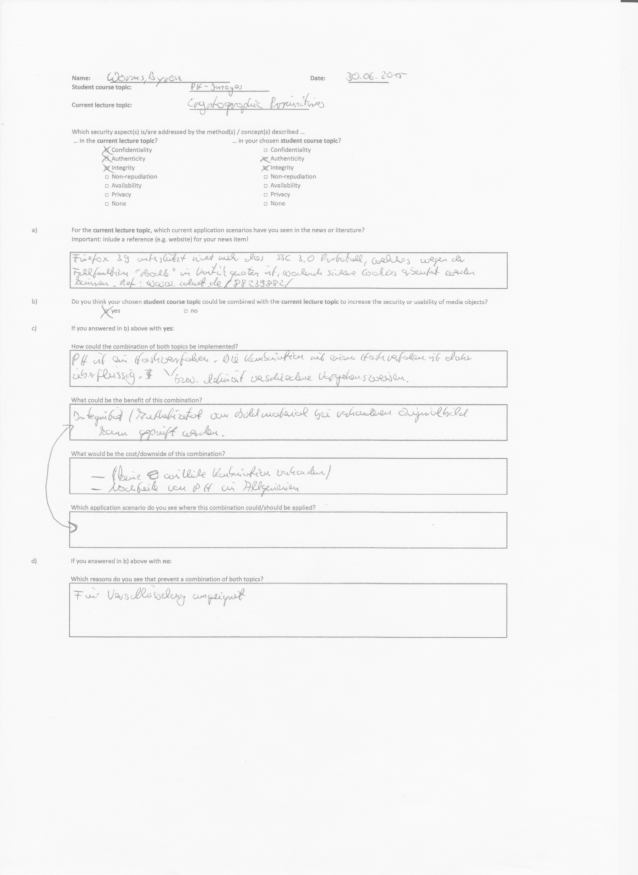
\includepdf[pages={1},scale=.85,pagecommand=\section{Discussion Tables}]{Pictures/table_primitives.pdf}
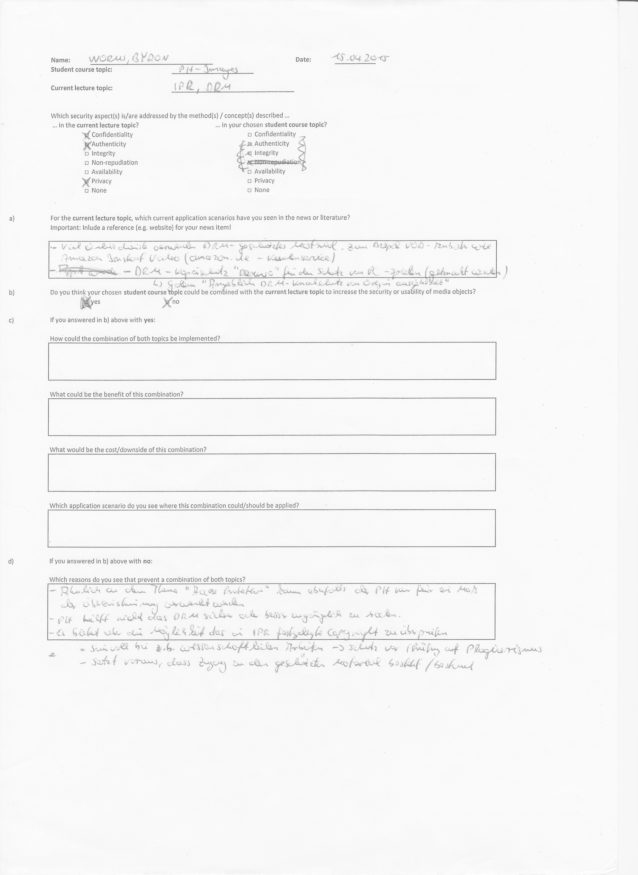
\includepdf[pages={1}]{Pictures/table_drm.pdf}
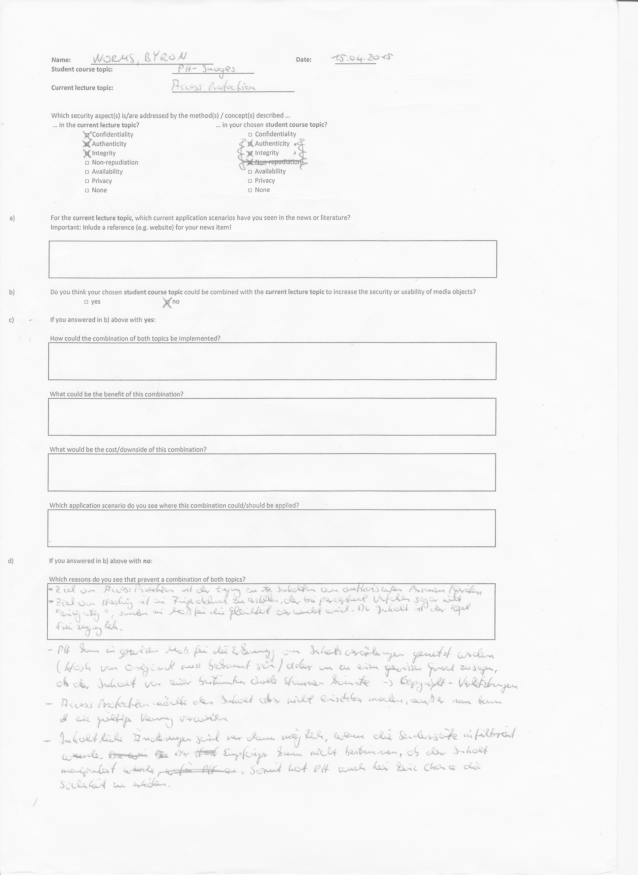
\includepdf[pages={1}]{Pictures/table_access.pdf}
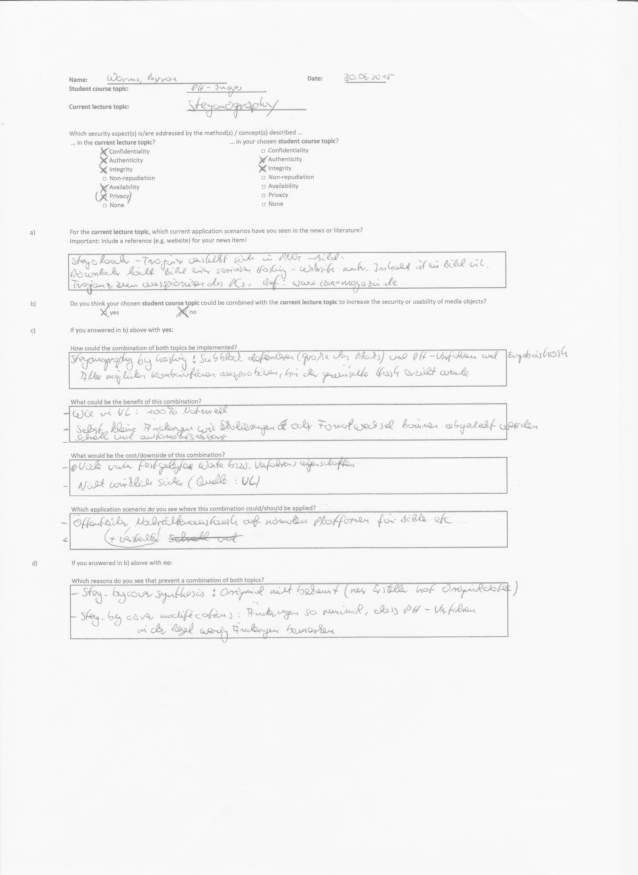
\includepdf[pages={1}]{Pictures/table_stego.pdf}
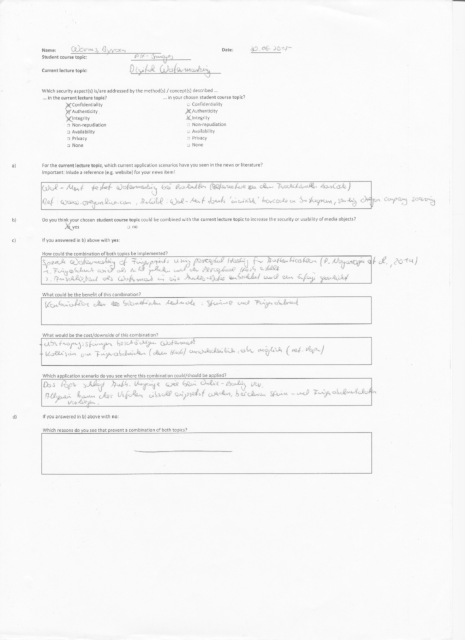
\includepdf[pages={1}]{Pictures/table_watermarking.pdf}
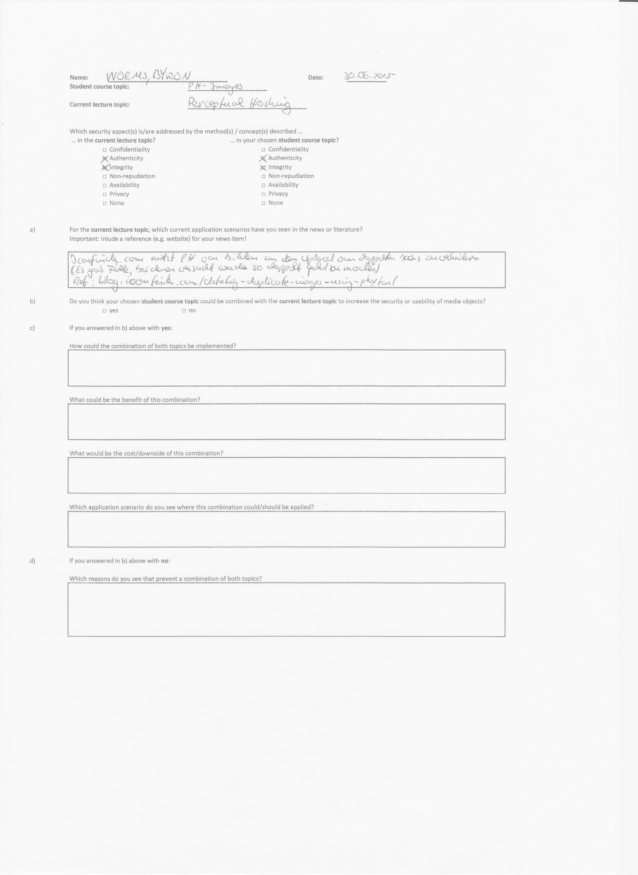
\includepdf[pages={1}]{Pictures/table_perceptual_hasing.pdf}
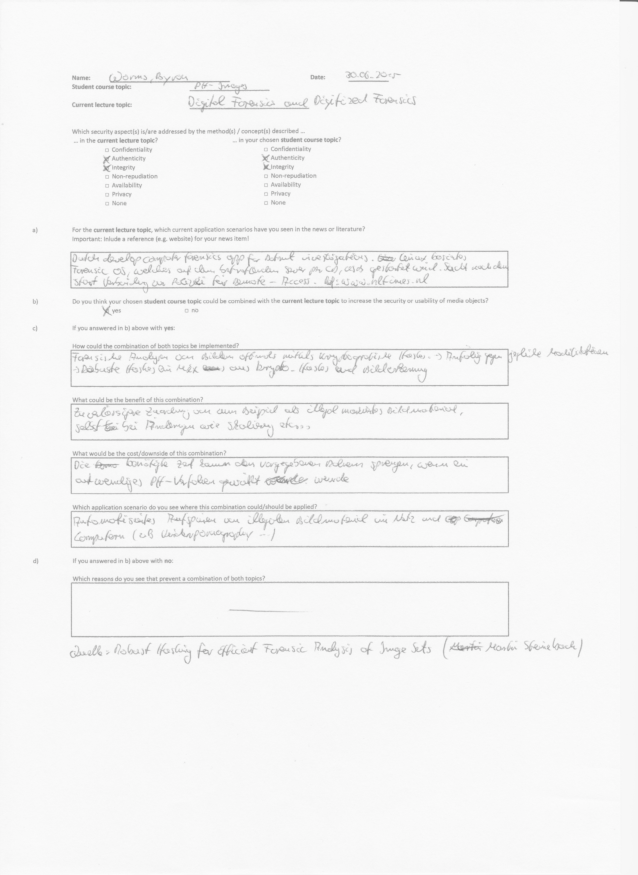
\includepdf[pages={1}]{Pictures/table_digital_forensics.pdf}	% Anhang E einbinden (Discussion Tables)
	\end{appendices}
\end{document}